\chapter{Introduction}
\label{:intro}


Range searching is one of the common types of problems which arise in everyday computer use. In a range search, we are given a set of objects and asked to identify those which satisfy some bounded criteria. Range searches can take many different forms: searching for email received between two dates, looking for restaurants near your present location, or identifying what a video game player should see on their screen in any one frame; these are all examples of range searches.

In computational geometry, range searching takes on a more abstract quality. 
Typically we are given an environment containing a set of geometric objects such as points, lines, circles, or boxes. 
A query is itself another well-defined geometric object, and our goal is to identify all elements of the environment contained within the query region.  
When addressing a range searching problem, we want to develop a method for preprocessing the input environment so that we can answer any query as efficiently as possible.
Given how common and flexible range searching is to such a wide range of practical computer science, it is not surprising to  find that a great deal of research has been expended in this area.  

In this thesis, we address the notion of \emph{Majority Range Searching}, which, to the best of our knowledge, has not been explored previously. In this setting, our goal is to identify all elements which intersect a query region by at least some fixed proportion of their own size (e.g., length, area, volume).  We contrast this problem from traditional range searching, which looks for objects which are entirely within a query region, and from intersection searching, which looks for any objects which have even a minimal intersection with a query region.

In this chapter, Section~\ref{:intro:motivation} begins by describing our motivation for this problem. In Section~\ref{:intro:problems} we describe the specific variations of the majority range problem that we will address in this thesis. In Section~\ref{:intro:related}, we discuss related problem domains, and contrast them to our own. Section~\ref{:intro:contributions} outlines the contributions made by this thesis.  We conclude the introduction by outlining the organization of the remainder of the thesis in Section~\ref{:intro:organization}.

%------------------------------------------------------------------------------%------------------------------------------------------------------------------
\section{Motivation}
\label{:intro:motivation}

The problem was inspired by the author's use of Microsoft OneNote. 
Using a digital pen, OneNote can be used much like a paper notebook, allowing the user to add handwriting, diagrams, equations, and any other such thing.
Unlike a paper notebook, OneNote also allows the user to select previous drawn objects in order to translate, scale, copy and otherwise manipulate what has been written.
Figure~\ref{fig:intro:onenote} shows some handwritten notes, as well as a diagram which has been partially selected.

\begin{figure}
\begin{center}
  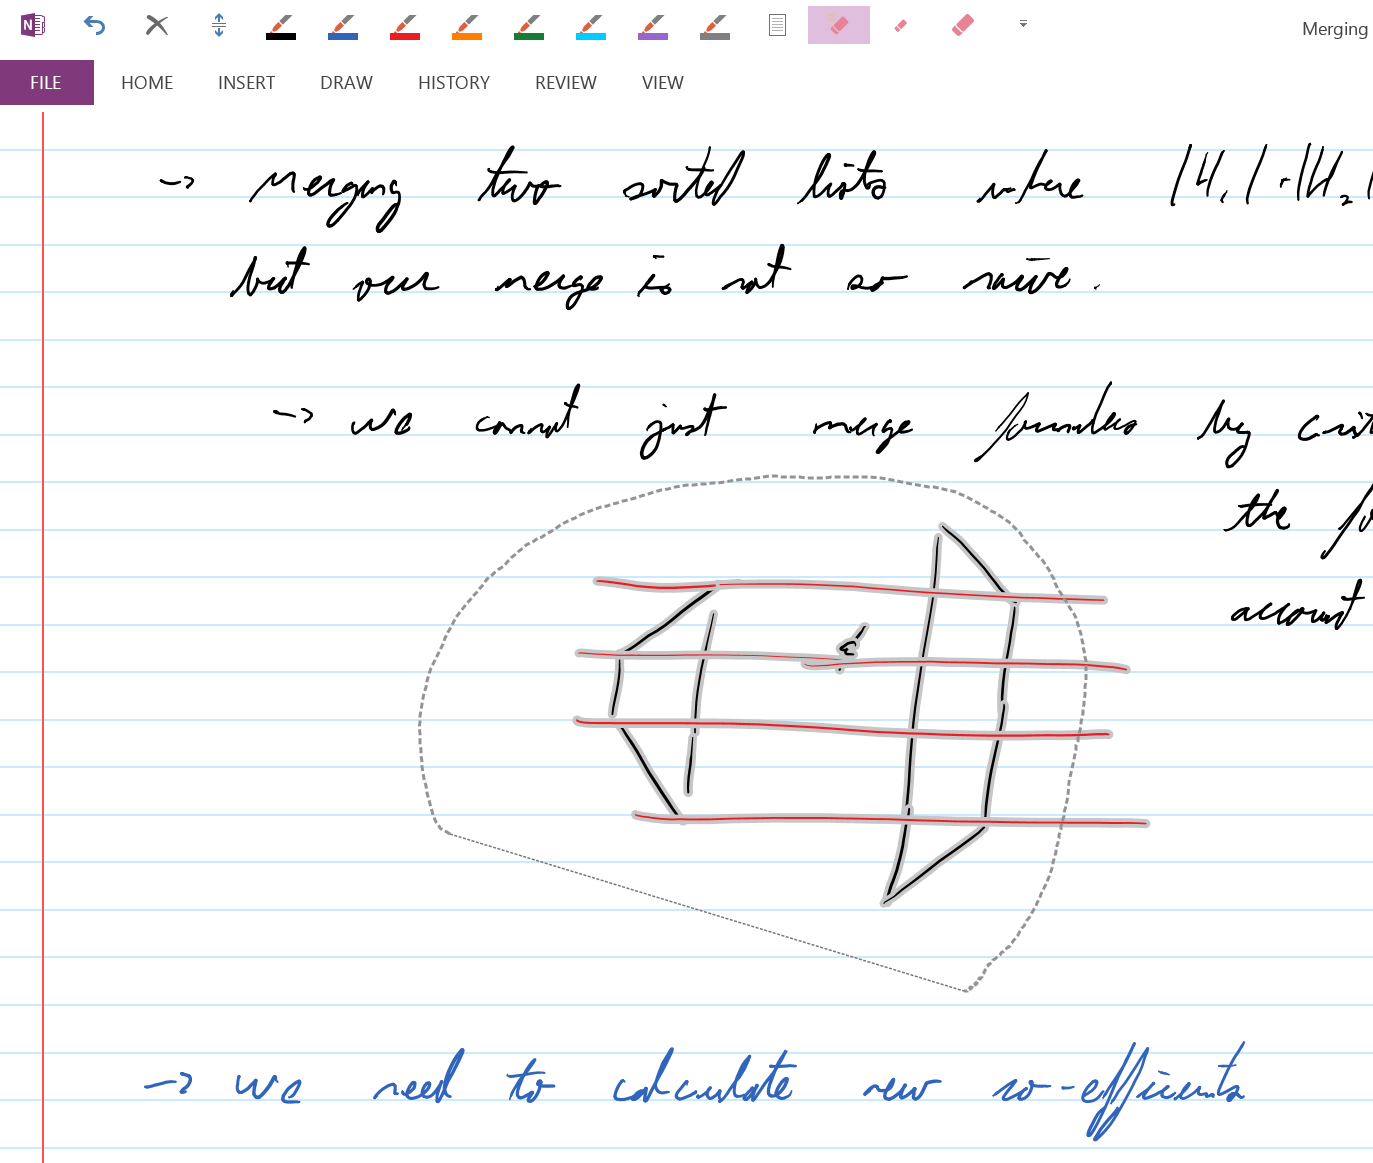
\includegraphics[width=0.50\textwidth]{figures/fig_onenote}
  \caption[An example of practical majority range searching]{An example of practical majority range searching in Microsoft OneNote. The line segments in the middle are selected but not entirely enclosed.}
  \label{fig:intro:onenote}
\end{center}
\end{figure}

Looking carefully at the figure, we can see that the even though the horizontal line segments have not been entirely enclosed by the selection tool, they nevertheless appear as part of the set of selected items.
This behaviour of selecting partially enclosed objects is described in a patent filed by Microsoft Corporation\cite{lassoselect} and is intended to ameliorate inherit problems with trying to select irregular shapes with an irregularly shaped selection region. 
From the patent:

\begin{quote}
[T]here is a need for a selection tool that will allow a user to conveniently select one or more graphical objects in their entirety, without requiring an inconvenient amount of precision from the user.
\end{quote}

\noindent Particularly with the rising popularity of touch and pen-enabled devices, this need will only increase.  
As we can see from the figure, OneNote already includes an implementation of a partial selection tool like the one described in the patent. 
Although the details of the implementation are proprietary, it becomes apparent while using the software that the implementation suffers from poor performance as more items are selected from denser pages.
It is from this observation that the work in this thesis was inspired.  
Although the problems that we will examine take place in a simpler setting than the patent describes, we will nevertheless develop an understanding of where the major challenges of this problem domain are found, as well as some techniques for addressing them.


%------------------------------------------------------------------------------%------------------------------------------------------------------------------
\section{Problem Statements}
\label{:intro:problems}

This thesis proposes algorithms for several different majority range query settings.  Each problem addresses a different type of geometric object to be queried, or a different type of query region.

\begin{enumerate}
\item Querying axis-parallel line segments with an axis-parallel rectangle.

\item Querying arbitrarily-oriented line segments with an axis-parallel rectangle.

\item Querying axis-parallel line segments with an arbitrarily-oriented slab.

\item Querying axis-parallel line segments with the intersection of two arbitrarily-oriented slabs. This problem is a generalization of querying axis-parallel segments with an arbitrarily-oriented rectangle.

\item Querying convex polygons with an arbitrarily-oriented rectangle.

\item Querying monotone polygons with an axis-parallel rectangle.
\end{enumerate}


%------------------------------------------------------------------------------%------------------------------------------------------------------------------
\section{Related Work}
\label{:intro:related}

\paragraph{Range Searching.} 
XXX TODO

\paragraph{Intersection Searching.} 
XXX TODO


%------------------------------------------------------------------------------
%------------------------------------------------------------------------------
\section{Summary of Contributions}
\label{:intro:contributions}

XXX TODO

A method for calculating the area of a convex polygon within a rectangle in $\BigOh{\log{n}}$ time with only
$\BigOh{n}$ preprocessing time and space. This immediately gives rise to a method to answer majority enclosure queries in the same time and space.

A method for calculating the area of a monotone polygon within a rectangle in $\BigOh{\log{n}}$ time with only
$\BigOh{n \log{n}}$ preprocessing time and space. As with the convex polygon case, this immediately gives a method for answering majority enclosure queries in the same time and space.


%------------------------------------------------------------------------------
%------------------------------------------------------------------------------
\section{Organization of the Thesis}
\label{:intro:organization}

The remainder of this thesis is organized in the following way. 
Chapter~\ref{:prelim} reviews existing data structures and range searching techniques which we utilize in our own contributions.
The next four chapters cover majority range searching queries on successively more sophisticated geometric objects, with Chapter~\ref{:rectangles} focusing on axis-parallel rectangles, Chapter~\ref{:slabs} on arbitrarily-oriented slabs, Chapter~\ref{:convexp} on convex polygons, and Chapter~\ref{:monotonep} on monotone polygons.
The thesis concludes with Chapter~\ref{:conclusion} which summarizes our contributions and future work presented in earlier chapters.
